%%%%%%%%%%%%%%%%%%%%%%%%%%%%%%%%%%%%%%%%%%%%%%%%%%%%%%%%%%%%%%%%%%%%%%%
%%%%%%%%%%%%%%%%%%%%%%%%%%%%%%%%%%%%%%%%%%%%%%%%%%%%%%%%%%%%%%%%%%%%%%%
\deelmetoef{Module 3}{Digitale afbeeldingen en video}{Module 3. Digitale afbeeldingen en video}{Oplossingen module 3}{Oplossingen module 3}
\label{sec:digafbvid}
%%%%%%%%%%%%%%%%%%%%%%%%%%%%%%%%%%%%%%%%%%%%%%%%%%%%%%%%%%%%%%%%%%%%%%%
%%%%%%%%%%%%%%%%%%%%%%%%%%%%%%%%%%%%%%%%%%%%%%%%%%%%%%%%%%%%%%%%%%%%%%%

\begin{samenvatting}
Het meten van je hartslag met de smartphone is gebaseerd op voor ons oog quasi onzichtbare kleurveranderingen in je vingertop. Deze kleurveranderingen filmen we met de smartphone camera, die ze wel kan zien. Om goed te begrijpen hoe we die kleurveranderingen precies kunnen detecteren, is het belangrijk de basisprincipes achter digitale afbeeldingen en video te begrijpen. Daar gaan we in deze module dieper op in.
\end{samenvatting}
%

%%%%%%%%%%%%%%%%%%%%%%%%%%%%%%%%%%%%%%%%%%%%%%%%%%%%%%%%%%%%%%%%%%%%%%%
\section{Digitale afbeeldingen}
\label{sec:Mod3_Sec1}
%%%%%%%%%%%%%%%%%%%%%%%%%%%%%%%%%%%%%%%%%%%%%%%%%%%%%%%%%%%%%%%%%%%%%%%
%

\subsection{Hoe zijn digitale afbeeldingen opgebouwd?}

Om jullie te laten kennis maken met de basisprincipes achter digitale afbeeldingen, raden we jullie aan het filmpje te bekijken dat je via de QR-code online kan terugvinden. \footnote{\url{https://www.youtube.com/watch?v=UBX2QQHlQ_I} of zoek \textquotedblleft Stand-up comedy about spreadsheet \textquotedblright op YouTube.} Bekijk zeker het stukje tussen minuut 2 en minuut 8. Het is een Engelstalig filmpje, maar je kan het ondertitelen (in het Engels) en eventueel ook vertraagd bekijken. 

\gewonefiguur{width=4cm}{module3/qrcode_youtubespreadsheets}

Het filmpje legt uit hoe digitale afbeeldingen opgebouwd zijn als een rooster. De vakjes uit het rooster noemen we \textquotedblleft pixels\textquotedblright. De term pixels komt uit het Engels en is een afkorting van \textquotedblleft picture elements \textquotedblright, \textquotedblleft foto-elementen\textquotedblright.

\gewonefiguur{width=\linewidth}{module3/voetballer-raster}

Elk pixel heeft een roodwaarde, een groenwaarde en een blauwwaarde. Met de combinatie van drie kleuren, nl. rood, groen en blauw, kan je quasi elke bestaande kleur genereren. Dit kan je een beetje vergelijken met een schilderspalet: een schilder mengt basiskleuren (rood, geel en blauw) tot hij de gewenste kleur bekomt. Bij een foto gebeurt iets vergelijkbaars: licht uit verschillende basiskleuren(rood, groen en blauw) mengt samen tot een nieuwe kleur.

De rood-, groen- en blauwwaarde van een pixel is steeds een getal tussen 0 en 255. Hoe kleiner het getal, hoe donkerder de kleur. Een roodwaarde van 0 komt dus overeen met een rood dat bijna zwart is. Omgekeerd: hoe groter het getal, hoe lichter de kleur. Een roodwaarde van 255 komt dus overeen met een rood dat bijna helemaal wit is. De drie getalwaarden voor rood, groen en zwart samen bepalen volledig de kleur die je zal zien. Dit drietal noemen we de RGB-waarde (R van rood/red, G van groen/green en B van blauw/blue) van de pixel.

\begin{oef}
	Hoeveel verschillende RGB-kleuren kan je genereren als de rood-, groen- en blauwwaarden steeds een waarde tussen 0 en 255 aannemen? 
\end{oef}
\oplos{Je kan $256 \cdot 256 \cdot 256 = 16 777 216$ verschillende kleuren genereren. Dit zijn wellicht meer kleuren dan jij met het blote oog kan onderscheiden.}

Hieronder zie je hoe een digitale afbeelding in een computer voorgesteld wordt: van elk pixel wordt bijgehouden hoeveel rood, groen en blauw die bevat. 

\gewonefiguur{width=\linewidth}{module3/voetballer-opgesplitst_RGB}

Je kan ook zelf experimenteren met de RGB-waarden van een foto. 

Via \url{http://makeanddo4d.com/spreadsheet/} of onderstaande QR-code kan je een foto omzetten in een Excel-werkblad. Inzoomen in het werkblad toont je de RBG-waarden van de inviduele pixels. Uitzoomen in het werkblad toont je de volledige foto. De resolutie van de foto, dit is de hoeveelheid detail of de scherpte, is weliswaar beperkt.

\gewonefiguur{width=4cm}{module3/qrcode_spreadsheetmaker}

\gewonefiguur{width=\linewidth}{module3/spreadsheetVb}

Als je de RGB waarden van enkele pixels aanpast en een beetje uitzoomt, zal je een andere kleur zien.


\subsection{Toepassing op de hartslagmonitor: roodwaarde berekenen in MIT App Inventor 2}

Voor de hartslagmonitor hebben we enkel de roodwaarde van het filmpje van je vingertop nodig. Deze waarden gaan we analyseren.

Gedurende 1 hartslag verandert je vingertop heel subtiel van kleur. 
Die verandering in roodwaarde van je vinger kan je met het blote oog niet detecteren, maar als je een filmpje maakt van je vinger, kan een computer of je smartphone die subtiele kleurverschillen w\'el waarnemen.

We maken een filmpje van onze vingertop. Dit filmpje registreert de kleurveranderingen van je vingertop ten gevolge van je hartslag. Een filmpje dat afspeelt is in feite niet meer dan een aantal foto's die heel snel na elkaar getoond worden. Hier gaan we in Sectie \ref{sec:Mod3_Sec2} straks verder op in. Als we het opgenomen filmpje splitsen in de achterliggende foto's en van elke foto bepalen \textquotedblleft hoe rood\textquotedblright \  die is dan kennen we de roodwaarde van je vingertop in functie van de tijd. Dit is een grafiek, die net zoals de grafiek in hieronder (die je opmat via \emph{Science Journal}) een piek heeft voor elke hartslag. Door het aantal pieken in een beperkt tijdsinterval (bv $15~s$) te tellen en dit aantal te herleiden naar het aantal pieken per minuut (bvb. door het aantal pieken in $15~s$ te vermenigvuldigen met vier), kan je de hartslag berekenen.

\gewonefiguur{width=.3\linewidth}{module1/metingScienceJournal}

Om het project tot een goed einde te brengen, moeten we dus \textquotedblleft de roodwaarde\textquotedblright\  van een foto kunnen berekenen. 
De roodwaarde van een foto zullen we bepalen als het gemiddelde van de roodwaarde van elke pixel van de foto.


\begin{opdracht}{Opdracht: roodwaarde van een foto bepalen in App Inventor 2}
	
		\begin{minipage}{.1\linewidth}
			
\includegraphics[width=1.5cm]{inputs/opdracht}
			\vspace{3cm}
		\end{minipage}
		\begin{minipage}{.5\linewidth}
			Bepaal de roodwaarde van een foto in App Inventor 2. Jouw opdracht luidt: kies de juiste blokken uit om ervoor te zorgen dat het indrukken van een knop resulteert in het berekenen van de roodwaarde van de foto. Het resultaat van die berekening dient te verschijnen in een label component. 
		\end{minipage}
		\begin{minipage}{.4\linewidth}
			\gewonefiguur{width=\linewidth}{module3/roodwaarde_canvas}
		\end{minipage}
		
	
		\begin{tabular}{c|L{8cm}|L{8cm}}
			& \multicolumn{1}{>{\centering\arraybackslash}m{80mm}|}{\textbf{DENK}}  & \multicolumn{1}{>{\centering\arraybackslash}m{80mm}}{\textbf{DOE}}  \\
			\hline
			1 & & Cre\"eer een nieuw project, genaamd \textquotedblleft Sommeer getallen\textquotedblright.  \\
			\hline
			2 & \emph{Ontwerper} view: & \\
			&  1. Welke componenten heb je nodig? & \vspace{2cm} \\
			&  2. Welke naam geef je aan iedere component? & \vspace{2cm} \\
			& & 3. Voeg een \hl{\texttt{canvas(E)/doek(NL)}} component. \vspace{0.3cm} \\
			& & 4. Upload een foto naar keuze en stel de foto in als achtergrond van het canvas. \vspace{0.3cm}\\
			& 5. Pas de afmetingen van het canvas aan zodat de verhoudingen van de foto goed zijn. \newline
			\emph{Tip:} Voor de meeste rechtopstaande foto's is de verhouding tussen de hoogte en de breedte 16:9 (voor liggende foto's 9:16). Als de hoogte van een rechtopstaande foto vastgelegd wordt op 200 pixels, moet de breedte dus ongeveer $\frac{9}{16}200$ pixels zijn om de oorspronkelijke verhouding te respecteren. \vspace{.3cm} & 5. hoogte: \hspace{4cm} pixels \newline \hspace{0.4cm} breedte: \hspace{4cm} pixels \\
			\end{tabular}
		
		Nu stappen we over naar de \hl{\emph{Blokken view}}. Zorg dat het indrukken van een knop resulteert in het berekenen van de gemiddelde roodwaarde van de foto. Het resultaat van die berekening dient te verschijnen in een label component.
		
		Op dit moment duiken we in het echte programmeerwerk. We geven je deze handige tips:
		
		\begin{itemize}
			\item \emph{Tip:} De canvas component heeft een methode/blok waarmee je de kleurwaarde van een pixel op breedte $x$ en hoogte $y$ in het rooster van de foto kan berekenen. 
			
			\item \emph{Tip:} Gebruik \hl{\texttt{Split color}} om de kleurwaarde van een foto op te splitsen in een lijst met drie elementen: de RGB-waarde.
			
			\item \emph{Tip:} Om de roodwaarde te bekomen, selecteer je het eerste element uit de lijst met de drie kleurwaarden. Je krijgt dus de R van de RGB-waarde.
			
			\item \emph{Tip:} Om de gemiddelde roodwaarde van een foto te berekenen, gebruik je twee for-lussen: \'e\'en lus loopt over alle pixels in de breedte van een foto ($x$ varieert), de andere lus loopt over alle pixels in de hoogte van de foto ($y$ varieert). De grenzen waarbinnen $x$ en $y$ vari\"eren, kan je bepalen a.d.h.v. de breedte en de hoogte van je canvas component.
			
			\item \emph{Tip:} om een gemiddelde van een rij getallen te berekenen, maak je eerst de som van alle getallen, en die som deel je vervolgens door het aantal getallen dat je opgeteld hebt:
			
			\begin{equation*}
			\text{Gemiddelde van 2, 7 en 10} = \frac{2+7+10}{3} = 6,33
			\end{equation*}
			
			Iets algemener, voor het gemiddelde van 5 willekeurige getallen:
			\begin{equation*}
			\overline{a_5} = \text{Gemiddelde van $a_1$, $a_2$, ..., $a_5$} = \frac{a_1+a_2+\ldots+a_5}{n} = \frac{\sum_{i=1}^{5} a_i}{5}
			\end{equation*}
			
			We  noteren het gemiddelde van 5 willekeurige getallen als $\overline{a}_5$. Het streepje boven de $\overline{a}$ duidt aan dat het om een gemiddelde gaat.
			
			Om een som van veel getallen kort te noteren, gebruiken we het sommatie-teken $\sum_{i=1}^{5}$.
			
			Nog algemener, voor het gemiddelde van $n$ willekeurige getallen:
			\begin{equation*}
			\overline{a_n} = \text{Gemiddelde van $a_1$, $a_2$, ..., $a_n$} = \frac{a_1+a_2+\ldots+a_n}{n} = \frac{\sum_{i=1}^{n} a_i}{n}
			\end{equation*}
			
		\end{itemize}
			
		\begin{tabular}{c|L{8cm}|L{8cm}}
			& \multicolumn{1}{>{\centering\arraybackslash}m{80mm}|}{\textbf{DENK}}  & \multicolumn{1}{>{\centering\arraybackslash}m{80mm}}{\textbf{DOE}}  \\
			\hline
			3 & \emph{Blokken} view & \\
			& 1. Hoe kan je de kleur van een pixel bekomen? (Kijk indien nodig bij de tips hierboven) & \vspace{2cm} \\
			& 2. Hoe extraheer je de roodwaarde uit een gegeven kleur? & \\  & & 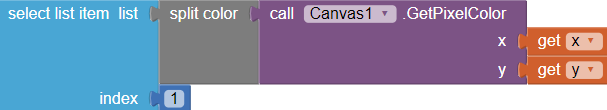
\includegraphics[width=\linewidth]{inputs/module3/roodwaarde_canvas_splitkleur}\\
			& 3. Hoe overloop je alle pixels van het canvas? & \vspace{2cm} \\
			& 4. Hoe bereken je het gemiddelde van de ge\"extraheerde roodwaarden? & \vspace{2cm}\\ 
		\end{tabular}
		
		Test de werking van je app grondig. 
		
		\begin{opmerking}
			De gemiddelde roodwaarde van een foto berekenen kan even duren!
			
			Daarom gaan we in de toekomst niet werken via deze omslachtige manier, maar we zullen dit oplossen door een apart blok te gebruiken dat een foto als input neemt en meteen de gemiddelde roodwaarde van de foto als output teruggeeft.
		\end{opmerking}
		
		\opdrachteindbalk
\end{opdracht}

%%%%%%%%%%%%%%%%%%%%%%%%%%%%%%%%%%%%%%%%%%%%%%%%%%%%%%%%%%%%%%%%%%%%%%%
\section{Digitale video}
\label{sec:Mod3_Sec2}
%%%%%%%%%%%%%%%%%%%%%%%%%%%%%%%%%%%%%%%%%%%%%%%%%%%%%%%%%%%%%%%%%%%%%%%
%

\subsection{Bewegende beelden}

In onderstaand filmpje (Engelstalig, met de mogelijkheid te ondertitelen en indien nodig te vertragen) worden de basisprincipes achter digitale video uitgelegd. \footnote{\url{https://www.youtube.com/watch?v=-1s-SuUQYs4} of zoek \text{The very basics of digital video} op YouTube.} 

\gewonefiguur{width=4cm}{module3/qrcode_youtubeDigitalVideo}

We vatten de inhoud van het filmpje hieronder nog even samen. Zoals eerder gezegd is digitale video een opeenvolging van digitale afbeeldingen, die snel na elkaar in beeld komen tegen een vaste snelheid.
De digitale afbeeldingen waaruit een video is opgebouwd, noemen we frames.
De snelheid waarmee frames na elkaar getoond worden is de frame rate, uitgedrukt in frames per seconde (of kortweg $fps$).
Onderzoek toonde aan dat een gemiddelde mens vanaf een snelheid van 24 $fps$ de individuele afbeeldingen als bewegende beelden zal waarnemen.

\begin{oef}
	Hoelang is elke afbeelding zichtbaar als afbeeldingen in een video elkaar opvolgen aan een snelheid van 24 $fps$? 
	En wat als de frame rate 30 $fps$ is?
\end{oef}
\oplos{Voor een frame rate van 24 $fps$ wordt elke afbeelding gedurende 0.042 $s$ (of 42 $ms$) getoond. Voor een frame rate van 30 $fps$ wordt elke afbeelding gedurende 0.033 $s$ (of 33 $ms$) getoond.}

\subsection{Afmetingen van een frame}

Elk frame heeft een breedte $B$ en een hoogte $H$, uitgedrukt in pixels.
We weten uit de vorige sectie dat een pixel in feite het kleinste bouwblokje van een digitale afbeelding is en dat elk pixel een RBG-waarde heeft.

\gewonefiguur{width=\linewidth}{module3/video_1}

De hoogte $H$ bepaalt de kwaliteit van het beeld. Hoe groter H, hoe scherper het beeld. Sommigen onder jullie hebben misschien al gehoord van standard definition (SD), high definition (HD) en full-HD beeldresolutie. 
De hoogte $H$ van de frames bepaalt of de beeldresolutie SD (als $H=480$ pixels), dan wel HD (als $H=720$ pixels), dan wel full-HD (als $H=1080$ pixels) is.

\subsection{Encodering}

Encodering is een proces dat gebruikt wordt om de grootte van de video te reduceren m.b.v. wiskundige bewerkingen. Met de grootte van de video bedoelen we hoeveel ruimte nodig is op je computer of smartphone om de video op te slaan. De video-grootte wordt meestal uitgedrukt in megabytes (MB). Ongecomprimeerde video is video waarop geen encodering is toegepast en neemt veel geheugenruimte in op je smartphone of computer. Encodering past een wiskundige bewerking toe op je video die ervoor zorgt dat de geheugenruimte beperkt blijft, zonder de kwaliteit van de video te veel aan te tasten. Afhankelijk van de gebruikte wiskundige bewerkingen krijgen we een ander encoderingsformaat. Vaak gebruikte encoderingsformaten zijn .mp4 en .mov, maar er bestaan nog veel andere formaten.


\begin{opdracht}{Opdracht: een willekeurig filmpje splitsen in aparte beelden}
Pluk een filmpje van het internet of maak zelf een filmpje. Gebruik de app \textquotedblleft Video naar afbeeldingen\textquotedblright \ om het filmpje te splitsen in opeenvolgende beelden.

\begin{opmerking}
	Het splitsen van video in afbeeldingen kan even duren!
\end{opmerking}

De app toont na het splitsen de aparte beelden. Deze beelden komen ook als aparte bestanden terecht op het geheugen van de smartphone. De map waar de beelden worden opgeslaan wordt ook weergegeven. Je kan deze beelden dus ook achteraf nog raadplegen of gebruiken.

\opdrachteindbalk

\end{opdracht}

Als je een willekeurig filmpje in beelden splitst, zie je hoe de beelden veranderen doorheen de tijd. Als de beelden snel genoeg na elkaar getoond worden, kan je oog de individuele beelden niet meer onderscheiden, waardoor je een continue beweging waarneemt.

\begin{opdracht}{Opdracht: een filmpje van je vingertop splitsen in foto's}
	Maak een filmpje van $15~s$ van de vingertop van je wijsvinger. Zet de flits van je smartphone aan. Leg je vinger op de lens van je camera en zorg dat je vinger de lens volledig bedekt. Het beeld zou volledig rood moeten zijn. Laat de camera gewoon rusten op je vingertop, je hoeft je vinger niet tegen de lens te duwen. 
	
	Splits het filmpje in foto's. 
	
	Zie jij de kleurverschillen ten gevolge van je hartslag?
	
	\opdrachteindbalk
\end{opdracht}


%%%%%%%%%%%%%%%%%%%%%%%%%%%%%%%%%%%%%%%%%%%%%%%%%%%%%%%%%%%%%%%%%%%%%%%
\section{Toepassing: de hartslagmonitor}
\label{sec:Mod3_Sec3}
%%%%%%%%%%%%%%%%%%%%%%%%%%%%%%%%%%%%%%%%%%%%%%%%%%%%%%%%%%%%%%%%%%%%%%%
%

\begin{opdracht}{Opdracht: roodwaarden bepalen en weergeven in een grafiek}
In de vorige twee opdrachten hebben jullie een filmpje gemaakt van je vingertop en dit splitst in afzonderlijke afbeeldingen. Daarnaast hebben jullie geleerd hoe je in App Inventor de roodwaarde van een individuele foto kan bepalen. Hier zullen we die twee combineren om de roodwaarden van de afzonderlijke foto's van je filmpje te bepalen. Die waarden slaan we op, en analyseren we in MS Excel, zodat we de hartslag kunnen berekenen.

\begin{enumerate}
	
	\item Maak een filmpje van $15~s$ van je vingertop of gebruik het filmpje uit de vorige opdracht.
	
	Zet de flits van je smartphone aan. Leg je vinger op de lens van je camera en zorg dat je vinger de lens volledig bedekt. Het beeld zou volledig rood moeten zijn. Laat de camera gewoon rusten op je vingertop, je hoeft je vinger niet tegen de lens te duwen.
	
	\item Splits het filmpje in foto's met de app \textquotedblleft Video naar afbeeldingen\textquotedblright.
	
	Als je dit in de vorige opdracht al gedaan hebt, mag je deze stap overslaan. Noteer de map waarin de afzonderlijke digitale afbeeldingen terecht kwamen, dit heb je straks nodig.
	
	\item Maak een nieuw project aan in MIT App Inventor 2 en geef het een passende naam, bv \texttt{Hartslagmonitor\_roodwaardenNaarExcel}. 
	
	\item \begin{minipage}{.1\linewidth}
		
\includegraphics[width=1.5cm]{inputs/opdracht}
		\vspace{2.5cm}
	\end{minipage}
	\begin{minipage}{.5\linewidth}
		Schrijf een app die, wanneer je de knop \hl{\texttt{BerekenRoodwaarden}} klikt, de roodwaarde van alle digitale afbeeldingen in de map berekent en toevoegt aan een lijst. Die lijst wordt vervolgens in een label en in een grafiek weergegeven.
	\end{minipage}
	\begin{minipage}{.3\linewidth}
		\gewonefiguur{width=5cm}{module3/roodwaardeGrafiek}
	\end{minipage}
	
	\begin{tabular}{c|L{8cm}|L{8cm}}
	& \multicolumn{1}{>{\centering\arraybackslash}m{80mm}|}{\textbf{DENK}}  & \multicolumn{1}{>{\centering\arraybackslash}m{80mm}}{\textbf{DOE}}  \\
	\hline
	1 & \emph{Ontwerper} view: & \\
	&  1. Welke componenten heb je nodig? & \vspace{2cm} \\
	&  2. Welke naam geef je aan iedere component? & \vspace{2cm} \\
	& & 3. We hebben een extensie gemaakt om extra functionaliteit toe te voegen die niet is ingebouwd in App Inventor 2 zelf. De extensie \hl{\texttt{extensieHartslagmonitor.aix}} voeg je toe in de tab \hl{\emph{Palet}} via \hl{\texttt{Importeer extensie}}. \vspace{.3cm}\\
	& & 4. Sleep de nieuwe componenten \texttt{RoodwaardeAfbeelding} en \texttt{GrafiekMaken} naar het afgebeelde smartphone-scherm. De componenten moeten onder de afgebeelde smartphone verschijnen. \vspace{.3cm}\\
	\end{tabular}
	
	\begin{tabular}{c|L{8cm}|L{8cm}}
	& \multicolumn{1}{>{\centering\arraybackslash}m{80mm}|}{\textbf{DENK}}  & \multicolumn{1}{>{\centering\arraybackslash}m{80mm}}{\textbf{DOE}}  \\
	\hline
	3 & \emph{Blokken} view: & \\
	&  1. De app moet toestemming hebben om bestanden op je smartphone te bekijken. Daarom zullen we bij het opstarten van de app vragen of de gebruiker toestemming geeft foto's, media en bestanden te openen. Voeg daarom het blok \hl{\texttt{Scherm $>$ Wanneer scherm initialiseer toe}}. Bij het opstarten van het scherm, moet de gebruiker om leestoestemming gevraagd worden. Gebruik daarvoor het blok \hl{\texttt{Scherm $>$ AskForPermission}} (Vertaling: vraag om toestemming). De \hl{\texttt{permissionName}} (vertaling: naam van de toestemming) is de tekst \textquotedblleft READ\_EXTERNAL\_STORAGE\textquotedblright. & \\
	& & \gewonefiguur{width=\linewidth}{module3/toestemming} \\
	& 2. Zorg ervoor dat klikken op de knop \hl{\texttt{BerekenRoodwaarden}}, resulteert in het berekenen van de roodwaarde van alle beelden in de video en deze toevoegt aan een lijst \texttt{roodwaardenLijst} \newline
	\emph{Hint:} in de extensie \hl{\texttt{RoodwaardeAfbeelding}} vind je hiervoor een nuttig blok. \vspace{.5cm} & \\
	& 3. Controleer of je effectief een lijst van roodwaarden bekomt door de variabele \hl{\texttt{roodwaardeLijst}} als label te tonen op het scherm van je smartphone. Tussen welke waarden verwacht je ongeveer dat de roodwaarden schommelen?
	\newline
	Bij het schrijven van code tonen we vaak tussentijdse resultaten op het scherm, om te controleren dat de code wel degelijk doet wat we verwachten. Ook dit is een onderdeel van het debuggen. & \\
	\end{tabular}

	\begin{tabular}{c|L{8cm}|L{8cm}}
	& \multicolumn{1}{>{\centering\arraybackslash}m{80mm}|}{\textbf{DENK}}  & \multicolumn{1}{>{\centering\arraybackslash}m{80mm}}{\textbf{DOE}}  \\
		\hline
	3 & \emph{Blokken} view: & \\
	& Nu heb je twee opties: 
	\begin{enumerate}
		\item de lijst van roodwaarden opslaan in een bestand om ze dan te analyseren als grafiek in MS Excel, OF
		\item in de app zelf de grafiek van roodwaarden maken
	\end{enumerate} 
	In beide gevallen maken we een grafiek waarin we het aantal pieken kunnen tellen en waaruit we de hartslag kunnen afleiden. Daarbij stellen we ons de volgende vragen:
	\begin{itemize}
		\item Welke grootheid staat op de horizontale as? Wat is de eenheid? \newline 
		\emph{Hint:} Er wordt aangeraden de tijd in milliseconden (ms) uit te zetten.
		\item Welke grootheid staat op de verticale as? Wat is de eenheid?
		\item Wat is de stapgrootte op de horizontale as? Hoe is de stapgrootte gerelateerd aan de frame rate?
		\item Wat is de maximale waarde op de horizontale as?
	\end{itemize}& \\
	& Om de tijd op de horizontale as correct te kunnen berekenen, moeten we de frame rate kennen. In de meeste nieuwe smartphones is de frame rate 30 $fps$. Dit is dus de standaardwaarde die we in de app zullen gebruiken.
	
	We moeten wel functionaliteit aan de app toevoegen die toelaat de frame rate te veranderen, mocht die niet overeenkomen met onze standaardwaarde van 30 $fps$. 
	
	In de vorige opdracht berekende je de frame rate voor de smartphone die jij gebruikte. Ga na of je de standaardwaarde van 30 $fps$ inderdaad moet veranderen.
	& Voeg daarom een tekstinput \hl{\texttt{fsInput}} en een knop \hl{\texttt{fsVeranderd}} toe aan je app. Wanneer je de tekstinput verandert, moet je de op knop \hl{\texttt{fsVeranderd}} drukken, waarna een globale variabele \texttt{fs} aangepast wordt. 
	\includegraphics[width=\linewidth]{inputs/module3/roodwaardeGrafiek_fsChanged}\\
	& 4a. Lijst van roodwaarden opslaan in MS Excel & \\
	\end{tabular}

	\begin{tabular}{c|L{8cm}|L{8cm}}
	& \multicolumn{1}{>{\centering\arraybackslash}m{80mm}|}{\textbf{DENK}}  & \multicolumn{1}{>{\centering\arraybackslash}m{80mm}}{\textbf{DOE}}  \\
	\hline
	& De lijst omgezet worden in een CSV tabel. CSV staat voor \emph{Comma Separated Value} wat we kunnen vertalen als \textquotedblleft waarden gescheiden door komma's\textquotedblright. Dit formaat komt vaak van pas om gegevens op te slaan in een tekstbestand, dat vervolgens eenvoudig kan ingelezen worden in MS Excel.
	& Voeg een \hl{\texttt{Bestand}}-component toe. \\
	& & 
\includegraphics[width=\linewidth]{inputs/module3/roodwaardeGrafiek_tocsv} \\
	& De \hl{\texttt{bestandsNaam}}-input mag je zelf kiezen, maar zorg dat de bestandsnaam eindigt op \textquotedblleft .csv\textquotedblright. Dit achtervoegsel na de punt heet de \textquotedblleft bestandsextensie \textquotedblright. Op basis van deze letters weet de computer met welk soort bestand het te maken heeft. De computer weet daarmee ook met welk programma hij het bestand moet openen wanneer we het willen bewerken of gebruiken. & \\
	\end{tabular}

	Het csv-bestand zou moeten opgeslaan worden op je smartphone in de map \emph{AppInventor/data}.
	
	Ga na dat het CSV-bestand inderdaad op de voorziene plaats en onder de voorziene naam opgeslaan is op je smartphone. Je kan navigeren door de bestanden op je smartphone via de app \textquotedblleft Bestanden\textquotedblright, die normaal gezien standaard ge\"installeerd is op Android smartphones.

	Kopieer het CSV-bestand van je smartphone naar je computer. Je kan dit doen door het bestand naar jezelf te mailen of het bestand op te laden naar je google drive en dan te downloaden vanaf je computer. Een alternatieve manier is het aansluiten van je smartphone aan op je computer via een USB-kabel en het bestand rechtstreeks te kopi\"eren. 
		
	Het CSV-bestand bevat zoals gezegd de roodwaarden van de digitale afbeeldingen waaruit de video bestaat. Je kan deze waarden inlezen in MS Excel. 
		
	\begin{itemize}
		\item Open een nieuwe MS Excel werkmap.
		\item Lees de gegevens in via het tabblad \hl{\emph{Gegevens} $>$ Van tekst}. Verplaats de roodwaarden naar kolom B. Voeg bovenaan een lege rij toe en geef kolom B een passende titel.
		\item Voeg de tijdstippen toe in kolom A. 
			
		De eerste foto werd geregistreerd op tijdstip 0,00. Gebruik de frame rate om de registratietijden van de volgende foto's toe te voegen. Ga indien nodig even terug naar oefening 1 in Sectie \ref{sec:Mod3_Sec2} om de duurtijd per foto $d$ te berekenen a.d.h.v. de frame rate.
			
		Als je de frame rate niet kent, kan je die berekenen. Hiervoor moet je weten hoelang je filmpje duurt. Duid dit aan met $D$. Dit kan je zien op je smartphone. In MS Excel kan je nagaan hoeveel foto's ge\"extraheerd werden. Dit duid je aan met $N$. De totale duur van de video $D$ gedeeld door het aantal foto's in de video $N$ geeft je het aantal seconden per foto/frame $d=\frac{D}{N}$. 
			
		\item Geef kolom A een passende titel.
			
		\item Maak een grafiek die de roodwaarde in functie van de tijd weergeeft. Welke kolom levert de waarden die op de $x$-as komen? En welke gegevens komen op de $y$-as?
			
		Hieronder zie je een voorbeeld.
			
		\gewonefiguur{width=\linewidth}{module3/MSExcel_graphRedValues}
			
		\item Tel het aantal pieken in de grafiek. Noteer ook hoelang het filmpje duurde. Gebruik beide gegevens om de hartslag, het aantal pieken per minuut, te berekenen.
			
		In de grafiek hierboven tellen we 19 pieken op 15 seconden. De hartslag is dus $19 \cdot 4 = 76$ bpm.
			
		\item Als de grafiek niet duidelijk genoeg is om pieken te kunnen tellen, maak dan een nieuw filmpje en herhaal de bovenstaande stappen. 
			
		Ga na welke factoren (bvb. flits aan/uit, hoe hard je op de lens drukt, hoe je je vinger houdt, ...) de kwaliteit van de meting be\"invloeden. Hou hiermee rekening als je later nog pogingen onderneemt om de hartslag te meten. Schrijf indien nodig je bevindingen ergens op.
		\end{itemize}
	
	\begin{tabular}{c|L{8cm}|L{8cm}}
	& \multicolumn{1}{>{\centering\arraybackslash}m{80mm}|}{\textbf{DENK}}  & \multicolumn{1}{>{\centering\arraybackslash}m{80mm}}{\textbf{DOE}}  \\
	\hline
	& 4b. Grafiek maken in de App Inventor 2 & \\ 
	& &
	Voeg een nieuwe knop \hl{\texttt{MaakGrafiek}} en een webviewer toe. \vspace{.3cm} \\
	& Maak een grafiek & \hl{\texttt{GrafiekMaken $>$ MaakLijnGrafiek}} \\
	& Denk na over: \begin{itemize}
		\item een passende titel
		\item de grootheid en eenheid op de horizontale as.
		\item de grootheid en eenheid op de verticale as.
		\item met welke stapgrootte de waarden op de $x$-as veranderen. Dit is de duurtijd per foto $d$ in milliseconden $ms$, die je in de vorige opdracht bepaalde.
		\item de \texttt{maximumXwaarde}, die het domein dat afgebeeld wordt op de $x$-as limiteert.
		\item welke waarden je wilt uitzetten in de grafiek, en
		\item in welke webviewer je de grafiek wilt weergeven.
	\end{itemize}
	Controleer dat de webviewer zichtbaar is en dat de grafiek correct wordt weergegeven alvorens verder te gaan!
	
	\begin{opmerking}
		Als je geen internet connectie hebt, zal je de grafiek niet kunnen weergeven! 
	\end{opmerking}
	\end{tabular}

\opdrachteindbalk

\begin{oef}
	Ken jij de bestandsextensies geassocieerd met volgende programma's?
		
	\begin{itemize}
		\item Word
		\item Excel
		\item Powerpoint
		\item Tekstbestand
	\end{itemize}
\end{oef}
\oplos{			
	\begin{itemize}
		\item Word $\rightarrow$ .docx
		\item Excel $\rightarrow$ .xlsx
		\item Powerpoint $\rightarrow$ .pptx
		\item Tekstbestand $\rightarrow$ .txt
	\end{itemize}
}
		
	
	
%	%	\begin{oef}
%	\begin{itemize}
%		\item Voeg de knoppen/labels/\ldots die je denkt nodig te hebben toe aan je scherm.
%		\item Indrukken van de knop \hl{\texttt{BerekenRoodwaarden}} dient de roodwaarden van alle afbeeldingen in de map te bepalen. Maak daarom eerst een lijst van alle afbeeldingen die in de genoteerde map opgeslaan zijn. 
%		
%		Hiervoor moet je een extensie gebruiken: \hl{\texttt{TaifunFile}}. Voeg in de \hl{\texttt{Designer}}-view de extensie toe in de tab \hl{\emph{Palet}} via \hl{\texttt{Importeer extensie}}. Sleep de extensie dan naar het afgebeelde smartphone-scherm. De extensie zou onder de afgebeelde smartphone moeten verschijnen. 
%		
%		In de \emph{Blocks}-view gebruik je het blok \hl{\texttt{TaifunFile - FileListAsync}} om alle bestanden in de genoteerde map op te lijsten. Dit blok gaat alle bestanden in de gevraagde map \hl{\texttt{directoryName}} en met de gevraagde extensie \hl{\texttt{extension}} oplijsten. Als je bij \hl{\texttt{includeSubDirectories}} \texttt{true} zet, worden ook submappen meegenomen in de oplijsting. Als \hl{\texttt{includeSubDirectories}} \texttt{false} is, wordt enkel de map zelf bekeken. 
%		
%		De oplijsting is \emph{asynchroon}: dat wil zeggen dat de smartphone andere processen kan uitvoeren tijdens de oplijsting. Maar dat betekent ook dat we niet weten wanneer de bestanden opgelijst zijn. Daarom gebruiken we ook het blok \hl{\texttt{TaifunFile - AfterFileListAsync}}. Dit blok treedt in werking wanneer alle bestanden opgelijst zijn, en dan kunnen we verder met onze berekeningen. Binnen dit blok hebben we een variabele \hl{\texttt{fileList}} waarin alle bestanden in de gevraagde map met de gevraagde extensie opgenomen zijn.
%		
%		De app moet toestemming hebben om bestanden op je smartphone te bekijken. Daarom zullen we bij het opstarten van de app vragen of de gebruiker toestemming geeft foto's, media en bestanden te openen. Voeg daarom het blok \hl{\texttt{Scherm $>$ Wanneer scherm initialiseer toe}}. Bij het opstarten van het scherm, moet de gebruiker om leestoestemming gevraagd worden. Gebruik daarvoor het blok \hl{\texttt{Scherm $>$ AskForPermission}} (Vertaling: vraag om toestemming). De \hl{\texttt{permissionName}} (vertaling: naam van de toestemming) is de tekst \textquotedblleft READ\_EXTERNAL\_STORAGE\textquotedblright.
%		
%		\gewonefiguur{width=.7\linewidth}{module3/toestemming}
%		
%		Ga even na af de oplijsting van de bestanden in de gevraagde map correct is verlopen. Dit doe je door de variabele \hl{\texttt{fileList}} als label te tonen op het scherm van je smartphone. Ga pas verder naar de volgende stap als je zeker bent dat dit juist is.
%		
%		\item Je zal merken dat de bestanden niet noodzakelijk in numeriek oplopende volgorde in \hl{\texttt{fileList}} staan. Daarom gaan we de lijst eerst sorteren. We willen immers eerst de roodwaarde van de eerste foto (met naam 001.jpg) berekenen, vervolgens die van de tweede foto (met naam 002.jpg), enzovoort.
%		
%		Om de lijst te sorteren, hebben we een tweede extensie gemaakt: \hl{\texttt{LijstVerwerken}}. Voeg de extensie toe zoals voorheen via \hl{\texttt{Importeer extensie}} en door de extensie naar het scherm van de afgebeelde smartphone te slepen.
%		
%		Gebruik het blok \hl{\texttt{LijstVerwerken $>$ SorteerLijst}} om de lijst te sorteren. Ga na dat dit correct gebeurde door de bekomen lijst als label te tonen op het scherm van je smartphone. Ga pas verder naar de volgende stap als dit correct werkt.
%		
%		\item Itereer over de items/bestanden in de lijst met gesorteerde bestanden en bereken van elk bestand (en dus van elke afbeelding) de roodwaarde. Voeg de bekomen roodwaarden telkens toe aan een lijst, die je bijvoorbeeld \hl{\texttt{roodwaardeLijst}} noemt.
%		
%		Controleer even of het proces de roodwaarden berekent door de variabele \hl{\texttt{roodwaardeLijst}} als label te tonen op het scherm van je smartphone. Ga pas verder naar de volgende stap als dit correct werkt.
%		
%		\item Ten slotte willen we de roodwaarden opslaan in een bestand dat we kunnen inlezen in MS Excel. Daarom moet de lijst omgezet worden in een CSV tabel. CSV staat voor \emph{Comma Separated Value} wat we kunnen vertalen als \textquotedblleft waarden gescheiden door komma's\textquotedblright. Dit formaat komt vaak van pas om gegevens op te slaan in een tekstbestand, dat vervolgens eenvoudig kan ingelezen worden in MS Excel.
%		
%		Voeg een nieuwe \hl{\texttt{File}}-component toe aan je scherm. De component zou onder de afgebeelde smartphone moeten verschijnen. 
%		
%		Gebruik het blok \hl{\texttt{File $>$ BewaarBestand}} en het blok \hl{\texttt{Lijst $>$ lijst naar .csv tabel}} om de lijst met roodwaarden (\hl{\texttt{roodwaardeLijst}}) eerst om te zetten in een CSV tabel. Die CSV tabel is de \hl{\texttt{tekst}} input van het blok \hl{\texttt{BewaarBestand}}. De \hl{\texttt{bestandsNaam}}-input mag je zelf kiezen, maar zorg dat de bestandsnaam eindigt op \textquotedblleft .csv\textquotedblright. Dit achtervoegsel na de punt heet de \textquotedblleft bestandsextensie \textquotedblright. Op basis van deze letters weet de computer met welk soort bestand het te maken heeft. De computer weet daarmee ook met welk programma hij het bestand moet openen wanneer we het willen bewerken of gebruiken.
%		
%		\begin{oef}
%			Ken jij de bestandsextensies geassocieerd met volgende programma's?
%			
%			\begin{itemize}
%				\item Word
%				\item Excel
%				\item Powerpoint
%				\item Tekstbestand
%			\end{itemize}
%		\end{oef}
%		\oplos{			
%			\begin{itemize}
%				\item Word $\rightarrow$ .docx
%				\item Excel $\rightarrow$ .xlsx
%				\item Powerpoint $\rightarrow$ .pptx
%				\item Tekstbestand $\rightarrow$ .txt
%			\end{itemize}
%		}
%		
%		Het csv-bestand zou moeten opgeslaan worden op je smartphone in de map A\emph{ppInventor/data}.
%		
%		Ga na dat het CSV-bestand inderdaad op de voorziene plaats en onder de voorziene naam opgeslaan is op je smartphone. Je kan navigeren door de bestanden op je smartphone via de app \textquotedblleft Bestanden\textquotedblright, die normaal gezien standaard ge\"installeerd is op Android smartphones.
%		
%		
%	\end{itemize}
%		\end{oef}
%		\oplos{\begin{itemize}
%				\item Knop \emph{BerekenRoodwaarden}, 
%			\end{itemize}
%	
%	\item Kopieer het CSV-bestand van je smartphone naar je computer. Je kan dit doen door het bestand naar jezelf te mailen of het bestand op te laden naar je google drive en dan te downloaden vanaf je computer. Een alternatieve manier is het aansluiten van je smartphone aan op je computer via een USB-kabel en het bestand rechtstreeks te kopi\"eren. 
%	
%	Het CSV-bestand bevat zoals gezegd de roodwaarden van de digitale afbeeldingen waaruit de video bestaat. Je kan deze waarden inlezen in MS Excel. 
%	
%	\begin{itemize}
%		\item Open een nieuwe MS Excel werkmap.
%		\item Lees de gegevens in via het tabblad \hl{\emph{Gegevens} $>$ Van tekst}. Verplaats de roodwaarden naar kolom B. Voeg bovenaan een lege rij toe en geef kolom B een passende titel.
%		\item Voeg de tijdstippen toe in kolom A. 
%		
%		De eerste foto werd geregistreerd op tijdstip 0,00. Gebruik de frame rate om de registratietijden van de volgende foto's toe te voegen. Ga indien nodig even terug naar oefening 1 in Sectie \ref{sec:Mod3_Sec2} om de duurtijd per foto $d$ te berekenen a.d.h.v. de frame rate.
%		
%		Als je de frame rate niet kent, kan je die berekenen. Hiervoor moet je weten hoelang je filmpje duurt. Duid dit aan met $D$. Dit kan je zien op je smartphone. In MS Excel kan je nagaan hoeveel foto's ge\"extraheerd werden. Dit duid je aan met $N$. De totale duur van de video $D$ gedeeld door het aantal foto's in de video $N$ geeft je het aantal seconden per foto/frame $d=\frac{D}{N}$. 
%		
%		\item Geef kolom A een passende titel.
%		
%		\item Maak een grafiek die de roodwaarde in functie van de tijd weergeeft. Welke kolom levert de waarden die op de $x$-as komen? En welke gegevens komen op de $y$-as?
%		
%		Hieronder zie je een voorbeeld.
%		
%		\gewonefiguur{width=\linewidth}{module3/MSExcel_graphRedValues}
%		
%		\item Tel het aantal pieken in de grafiek. Noteer ook hoelang het filmpje duurde. Gebruik beide gegevens om de hartslag, het aantal pieken per minuut, te berekenen.
%		
%		In de grafiek hierboven tellen we 19 pieken op 15 seconden. De hartslag is dus $19 \cdot 4 = 76$ bpm.
%		
%		\item Als de grafiek niet duidelijk genoeg is om pieken te kunnen tellen, maak dan een nieuw filmpje en herhaal de bovenstaande stappen. 
%		
%		Ga na welke factoren (bvb. flits aan/uit, hoe hard je op de lens drukt, hoe je je vinger houdt, ...) de kwaliteit van de meting be\"invloeden. Hou hiermee rekening als je later nog pogingen onderneemt om de hartslag te meten. Schrijf indien nodig je bevindingen ergens op.
%	\end{itemize}	
	
\end{enumerate}
	
%\begin{enumerate}
%	
%	\item Maak een filmpje van $15~s$ van je vingertop of gebruik het filmpje uit de vorige opdracht.
%	
%	Zet de flits van je smartphone aan. Leg je vinger op de lens van je camera en zorg dat je vinger de lens volledig bedekt. Het beeld zou volledig rood moeten zijn. Laat de camera gewoon rusten op je vingertop, je hoeft je vinger niet tegen de lens te duwen.
%	
%	\item Splits het filmpje in foto's met de app \textquotedblleft Video naar afbeeldingen\textquotedblright.
%	
%	Als je dit in de vorige opdracht al gedaan hebt, mag je deze stap overslaan. Noteer de map waarin de afzonderlijke digitale afbeeldingen terecht kwamen, dit heb je straks nodig.
%	
%	\item Maak een nieuw project aan in MIT App Inventor 2 en geef het een passende naam, bv \texttt{Hartslagmonitor\_roodwaardenNaarExcel}. 
%	
%	\item Schrijf een app die, wanneer je de knop \hl{\texttt{BerekenRoodwaarden}} klikt, de roodwaarde van alle digitale afbeeldingen in de map berekent en toevoegt aan een lijst. Zet vervolgens deze lijst om naar een CSV-tabel en sla de tabel op op je smartphone.
%
%	
%%	\begin{oef}
%		\begin{itemize}
%			\item Voeg de knoppen/labels/\ldots die je denkt nodig te hebben toe aan je scherm.
%			\item Indrukken van de knop \hl{\texttt{BerekenRoodwaarden}} dient de roodwaarden van alle afbeeldingen in de map te bepalen. Maak daarom eerst een lijst van alle afbeeldingen die in de genoteerde map opgeslaan zijn. 
%			
%			Hiervoor moet je een extensie gebruiken: \hl{\texttt{TaifunFile}}. Voeg in de \hl{\texttt{Designer}}-view de extensie toe in de tab \hl{\emph{Palet}} via \hl{\texttt{Importeer extensie}}. Sleep de extensie dan naar het afgebeelde smartphone-scherm. De extensie zou onder de afgebeelde smartphone moeten verschijnen. 
%			
%			In de \emph{Blocks}-view gebruik je het blok \hl{\texttt{TaifunFile - FileListAsync}} om alle bestanden in de genoteerde map op te lijsten. Dit blok gaat alle bestanden in de gevraagde map \hl{\texttt{directoryName}} en met de gevraagde extensie \hl{\texttt{extension}} oplijsten. Als je bij \hl{\texttt{includeSubDirectories}} \texttt{true} zet, worden ook submappen meegenomen in de oplijsting. Als \hl{\texttt{includeSubDirectories}} \texttt{false} is, wordt enkel de map zelf bekeken. 
%
%			De oplijsting is \emph{asynchroon}: dat wil zeggen dat de smartphone andere processen kan uitvoeren tijdens de oplijsting. Maar dat betekent ook dat we niet weten wanneer de bestanden opgelijst zijn. Daarom gebruiken we ook het blok \hl{\texttt{TaifunFile - AfterFileListAsync}}. Dit blok treedt in werking wanneer alle bestanden opgelijst zijn, en dan kunnen we verder met onze berekeningen. Binnen dit blok hebben we een variabele \hl{\texttt{fileList}} waarin alle bestanden in de gevraagde map met de gevraagde extensie opgenomen zijn.
%			
%			De app moet toestemming hebben om bestanden op je smartphone te bekijken. Daarom zullen we bij het opstarten van de app vragen of de gebruiker toestemming geeft foto's, media en bestanden te openen. Voeg daarom het blok \hl{\texttt{Scherm $>$ Wanneer scherm initialiseer toe}}. Bij het opstarten van het scherm, moet de gebruiker om leestoestemming gevraagd worden. Gebruik daarvoor het blok \hl{\texttt{Scherm $>$ AskForPermission}} (Vertaling: vraag om toestemming). De \hl{\texttt{permissionName}} (vertaling: naam van de toestemming) is de tekst \textquotedblleft READ\_EXTERNAL\_STORAGE\textquotedblright.
%			
%			\gewonefiguur{width=.7\linewidth}{module3/toestemming}
%			
%			Ga even na af de oplijsting van de bestanden in de gevraagde map correct is verlopen. Dit doe je door de variabele \hl{\texttt{fileList}} als label te tonen op het scherm van je smartphone. Ga pas verder naar de volgende stap als je zeker bent dat dit juist is.
%			
%			\item Je zal merken dat de bestanden niet noodzakelijk in numeriek oplopende volgorde in \hl{\texttt{fileList}} staan. Daarom gaan we de lijst eerst sorteren. We willen immers eerst de roodwaarde van de eerste foto (met naam 001.jpg) berekenen, vervolgens die van de tweede foto (met naam 002.jpg), enzovoort.
%			
%			Om de lijst te sorteren, hebben we een tweede extensie gemaakt: \hl{\texttt{LijstVerwerken}}. Voeg de extensie toe zoals voorheen via \hl{\texttt{Importeer extensie}} en door de extensie naar het scherm van de afgebeelde smartphone te slepen.
%			
%			Gebruik het blok \hl{\texttt{LijstVerwerken $>$ SorteerLijst}} om de lijst te sorteren. Ga na dat dit correct gebeurde door de bekomen lijst als label te tonen op het scherm van je smartphone. Ga pas verder naar de volgende stap als dit correct werkt.
%			
%			\item Itereer over de items/bestanden in de lijst met gesorteerde bestanden en bereken van elk bestand (en dus van elke afbeelding) de roodwaarde. Voeg de bekomen roodwaarden telkens toe aan een lijst, die je bijvoorbeeld \hl{\texttt{roodwaardeLijst}} noemt.
%			
%			Controleer even of het proces de roodwaarden berekent door de variabele \hl{\texttt{roodwaardeLijst}} als label te tonen op het scherm van je smartphone. Ga pas verder naar de volgende stap als dit correct werkt.
%			
%			\item Ten slotte willen we de roodwaarden opslaan in een bestand dat we kunnen inlezen in MS Excel. Daarom moet de lijst omgezet worden in een CSV tabel. CSV staat voor \emph{Comma Separated Value} wat we kunnen vertalen als \textquotedblleft waarden gescheiden door komma's\textquotedblright. Dit formaat komt vaak van pas om gegevens op te slaan in een tekstbestand, dat vervolgens eenvoudig kan ingelezen worden in MS Excel.
%			
%			Voeg een nieuwe \hl{\texttt{File}}-component toe aan je scherm. De component zou onder de afgebeelde smartphone moeten verschijnen. 
%			
%			Gebruik het blok \hl{\texttt{File $>$ BewaarBestand}} en het blok \hl{\texttt{Lijst $>$ lijst naar .csv tabel}} om de lijst met roodwaarden (\hl{\texttt{roodwaardeLijst}}) eerst om te zetten in een CSV tabel. Die CSV tabel is de \hl{\texttt{tekst}} input van het blok \hl{\texttt{BewaarBestand}}. De \hl{\texttt{bestandsNaam}}-input mag je zelf kiezen, maar zorg dat de bestandsnaam eindigt op \textquotedblleft .csv\textquotedblright. Dit achtervoegsel na de punt heet de \textquotedblleft bestandsextensie \textquotedblright. Op basis van deze letters weet de computer met welk soort bestand het te maken heeft. De computer weet daarmee ook met welk programma hij het bestand moet openen wanneer we het willen bewerken of gebruiken.
%			
%			\begin{oef}
%			Ken jij de bestandsextensies geassocieerd met volgende programma's?
%						
%			\begin{itemize}
%			\item Word
%			\item Excel
%			\item Powerpoint
%			\item Tekstbestand
%			\end{itemize}
%			\end{oef}
%			\oplos{			
%			\begin{itemize}
%					\item Word $\rightarrow$ .docx
%					\item Excel $\rightarrow$ .xlsx
%					\item Powerpoint $\rightarrow$ .pptx
%					\item Tekstbestand $\rightarrow$ .txt
%			\end{itemize}
%			}
%			
%			Het csv-bestand zou moeten opgeslaan worden op je smartphone in de map A\emph{ppInventor/data}.
%			
%			Ga na dat het CSV-bestand inderdaad op de voorziene plaats en onder de voorziene naam opgeslaan is op je smartphone. Je kan navigeren door de bestanden op je smartphone via de app \textquotedblleft Bestanden\textquotedblright, die normaal gezien standaard ge\"installeerd is op Android smartphones.
%			
%			
%		\end{itemize}
%%	\end{oef}
%%	\oplos{\begin{itemize}
%%			\item Knop \emph{BerekenRoodwaarden}, 
%%		\end{itemize}
%	
%	\item Kopieer het CSV-bestand van je smartphone naar je computer. Je kan dit doen door het bestand naar jezelf te mailen of het bestand op te laden naar je google drive en dan te downloaden vanaf je computer. Een alternatieve manier is het aansluiten van je smartphone aan op je computer via een USB-kabel en het bestand rechtstreeks te kopi\"eren. 
%	
%	Het CSV-bestand bevat zoals gezegd de roodwaarden van de digitale afbeeldingen waaruit de video bestaat. Je kan deze waarden inlezen in MS Excel. 
%	
%	\begin{itemize}
%		\item Open een nieuwe MS Excel werkmap.
%		\item Lees de gegevens in via het tabblad \hl{\emph{Gegevens} $>$ Van tekst}. Verplaats de roodwaarden naar kolom B. Voeg bovenaan een lege rij toe en geef kolom B een passende titel.
%		\item Voeg de tijdstippen toe in kolom A. 
%		
%		De eerste foto werd geregistreerd op tijdstip 0,00. Gebruik de frame rate om de registratietijden van de volgende foto's toe te voegen. Ga indien nodig even terug naar oefening 1 in Sectie \ref{sec:Mod3_Sec2} om de duurtijd per foto $d$ te berekenen a.d.h.v. de frame rate.
%		
%		Als je de frame rate niet kent, kan je die berekenen. Hiervoor moet je weten hoelang je filmpje duurt. Duid dit aan met $D$. Dit kan je zien op je smartphone. In MS Excel kan je nagaan hoeveel foto's ge\"extraheerd werden. Dit duid je aan met $N$. De totale duur van de video $D$ gedeeld door het aantal foto's in de video $N$ geeft je het aantal seconden per foto/frame $d=\frac{D}{N}$. 
%		
%		\item Geef kolom A een passende titel.
%		
%		\item Maak een grafiek die de roodwaarde in functie van de tijd weergeeft. Welke kolom levert de waarden die op de $x$-as komen? En welke gegevens komen op de $y$-as?
%		
%		Hieronder zie je een voorbeeld.
%		
%		\gewonefiguur{width=\linewidth}{module3/MSExcel_graphRedValues}
%		
%		\item Tel het aantal pieken in de grafiek. Noteer ook hoelang het filmpje duurde. Gebruik beide gegevens om de hartslag, het aantal pieken per minuut, te berekenen.
%		
%		In de grafiek hierboven tellen we 19 pieken op 15 seconden. De hartslag is dus $19 \cdot 4 = 76$ bpm.
%		
%		\item Als de grafiek niet duidelijk genoeg is om pieken te kunnen tellen, maak dan een nieuw filmpje en herhaal de bovenstaande stappen. 
%		
%		Ga na welke factoren (bvb. flits aan/uit, hoe hard je op de lens drukt, hoe je je vinger houdt, ...) de kwaliteit van de meting be\"invloeden. Hou hiermee rekening als je later nog pogingen onderneemt om de hartslag te meten. Schrijf indien nodig je bevindingen ergens op.
%	\end{itemize}	
%
%\end{enumerate}
	
\end{opdracht}

%\begin{opdracht}{Opdracht: roodwaarden bepalen en weergeven in de app}
%	In de vorige opdracht konden we voor het eerst onze hartslag bepalen o.b.v. een opgenomen video. De omweg via MS Excel is wel een beetje vervelend. In deze opdracht wijzigen we de app uit de vorige opdracht, zodat we de grafiek rechtstreeks in onze app kunnen maken en bekijken.
%	
%	\begin{enumerate}
%		\item Kopieer het vorige project en geef het een passende naam, bv \\
%		\texttt{Hartslagmonitor\_roodwaardeNaarGrafiek}. 
%		\item Om de tijd op de horizontale as correct te kunnen berekenen, moeten we de frame rate kennen. In de meeste nieuwe smartphones is de frame rate 30 $fps$. Dit is dus de standaardwaarde die we in de app zullen gebruiken.
%		
%		We moeten wel functionaliteit aan de app toevoegen die toelaat de frame rate te veranderen, mocht die niet overeenkomen met onze standaardwaarde van 30 $fps$. Voeg daarom een tekstinput \hl{\texttt{fsInput}} en een knop \hl{\texttt{fsVeranderd}} toe aan je app. Wanneer je de tekstinput verandert, moet je de op knop \hl{\texttt{fsVeranderd}} drukken, waarna een globale variabele \texttt{fs} aangepast wordt.
%		
%		In de vorige opdracht berekende je de frame rate voor de smartphone die jij gebruikte. Ga na of je de standaardwaarde van 30 $fps$ inderdaad moet veranderen.
%		
%		\item Voeg een nieuwe knop \hl{\texttt{MaakGrafiek}} en een webviewer toe. Voeg ook de extensie \hl{\texttt{GrafiekMaken}} toe door de extensie te importeren en dan de componenten te slepen naar het afgebeelde smartphonescherm.
%		
%		Gebruik het blok \hl{\texttt{GrafiekMaken $>$ MaakLijnGrafiek}} om een lijngrafiek te maken. Je kan de grafiek een titel, $x$- en $y$-labels geven. De input \texttt{stapgrootteX} geeft aan met welke stapgrootte de waarden op de $x$-as veranderen. Dit is de duurtijd per foto $d$, die je in de vorige opdracht bepaalde. Gebruik de duurtijd per foto in milliseconden $ms$. De input \texttt{maximumXwaarde} limiteert het domein dat afgebeeld wordt op de $x$-as. Ten slotte moet je meegeven welke waarden je wilt uitzetten in de grafiek, en in welke webviewer je de grafiek wilt weergeven.
%		
%		Controleer dat de webviewer zichtbaar is en dat de grafiek correct wordt weergegeven alvorens verder te gaan!
%		
%		\begin{opmerking}
%			Als je geen internet connectie hebt, zal je de grafiek niet kunnen weergeven! 
%		\end{opmerking}
%	\end{enumerate}
%\end{opdracht}
	


